\documentclass{article}

\usepackage[english]{babel}
\usepackage[letterpaper,top=2cm,bottom=2cm,left=3cm,right=3cm,marginparwidth=1.75cm]{geometry}

\usepackage{amsmath}
\usepackage{graphicx}
\usepackage[colorlinks=true, allcolors=blue]{hyperref}

\title{Wormhole Attack Analysis}
\author{Nikola Valesova}

\begin{document}
\maketitle

\section{Introduction}

A hack of the Wormhole Network, a popular cross-chain protocol, took place on 2 February 2022 when an unknown hacker exploited a vulnerability in the Wormhole Network. The attack resulted in one of the five largest crypto hacks of all time after the attacker successfully made close to \$325 million. \cite{chainanalysis}

The attacker made use of a security flaw that had been fixed in the latest commit of the project's GitHub repository, the new changes, however, had not yet been deployed to the project itself and thus revealed a possibility to bypass the security measures. \cite{the_verge}

To carry out the attack, the attacker managed to forge a valid signature for a transaction that allowed them to freely mint 120,000 WETH — a “wrapped” Ethereum equivalent on the Solana blockchain, with value equivalent to \$325 million at the time of the theft — without first inputting an equivalent amount. This was then exchanged for around \$250 million in Ethereum that was sent from Wormhole to the hackers’ account, effectively liquidating a large amount of the platform’s Ethereum funds that were being held as collateral for transactions on the Solana blockchain. \cite{the_verge}

\section{Attack overview}

From a high-level perspective, the attack and its preceding and succeeding actions can be described by five transactions. A diagram of the parties and transactions involved can be seen on the Chainalysis Reactor graph \ref{fig:reactor_graph}. The content of this section has been written on the basis of information in an article by ChainAnalysis \cite{chainanalysis}.

\begin{figure}[ht!]
\centering
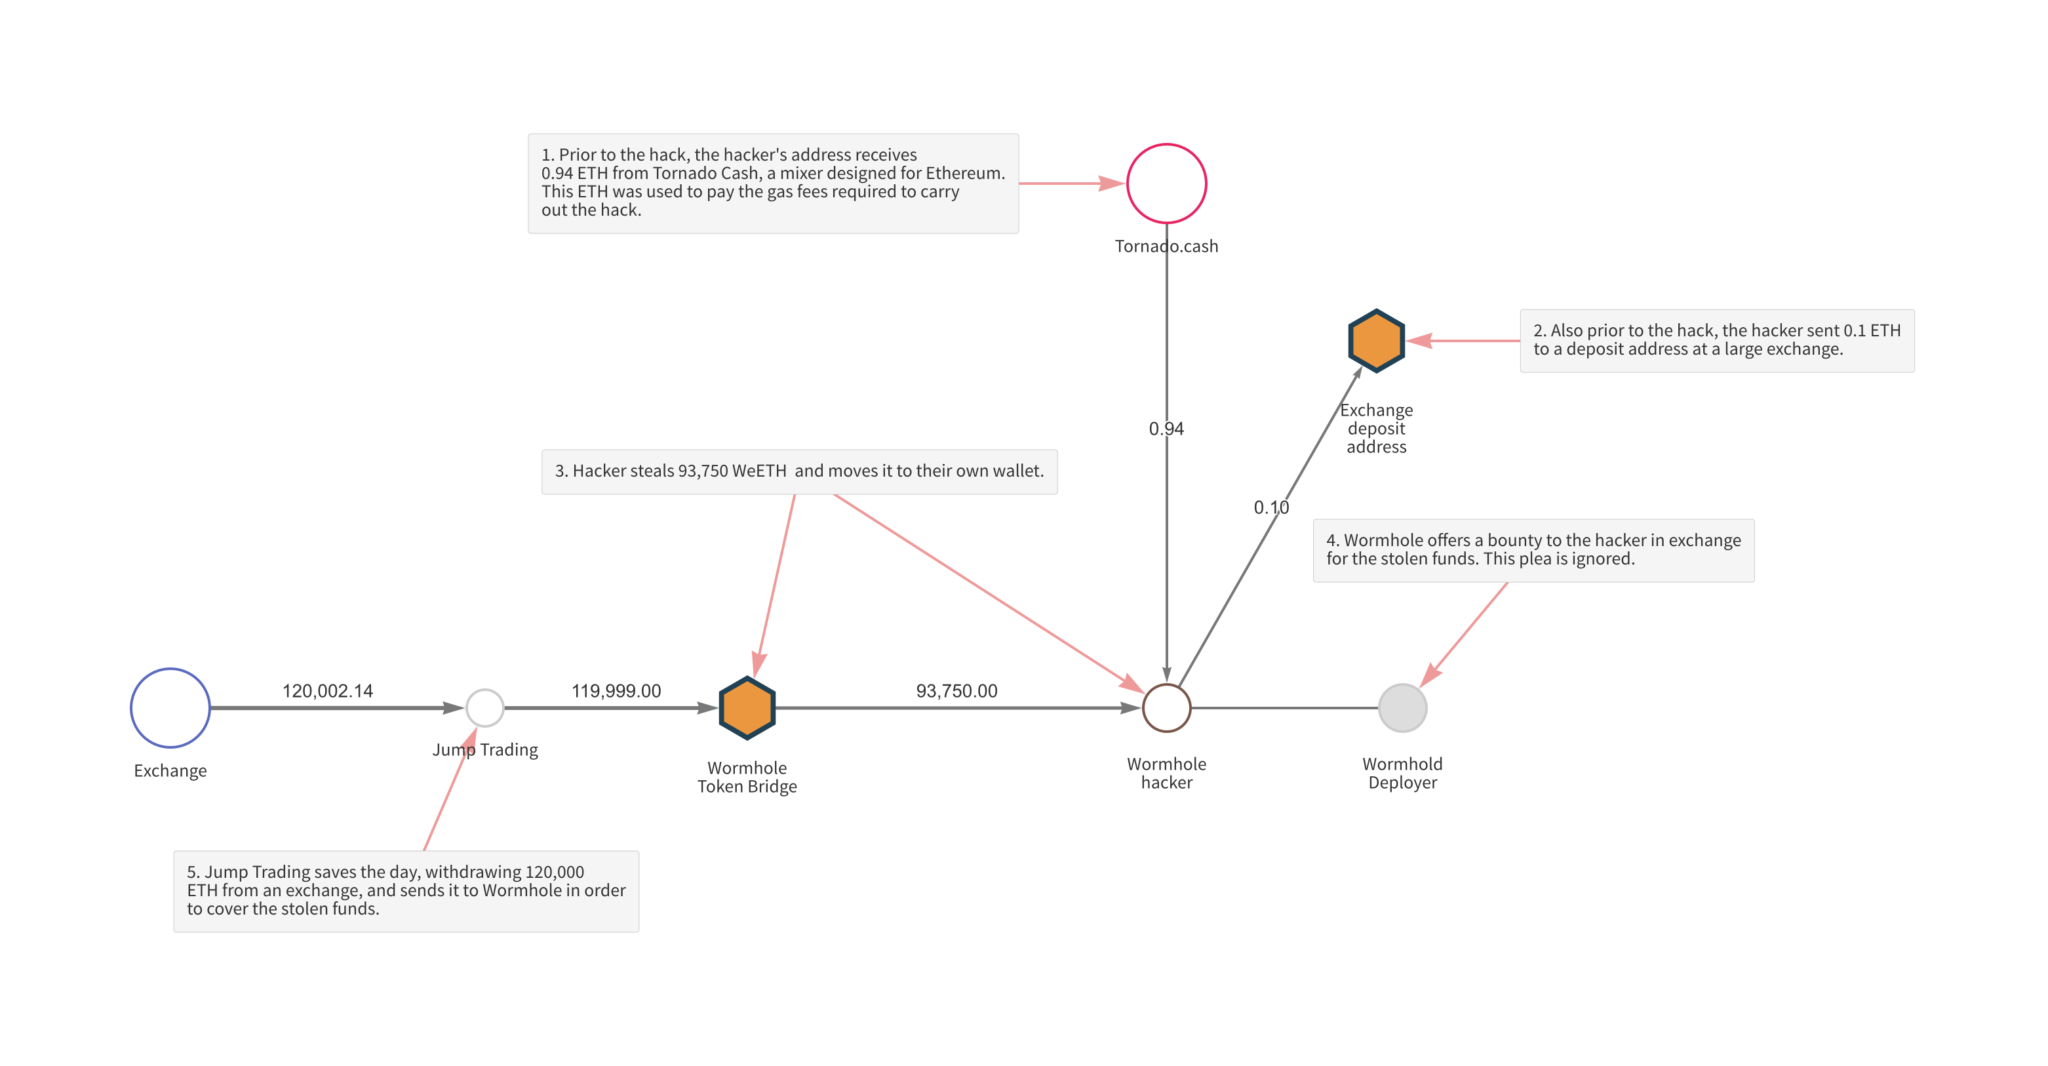
\includegraphics[width=\textwidth]{img/Wormhole_hack.png}
\caption{\label{fig:reactor_graph}Chainalysis Reactor graph of the Wormhole hack}
\end{figure}

\begin{enumerate}
\item Hacker's address receives 0.94 ETH from Tornado Cash

The first transaction happens in preparation for the attack. The hacker uses Tornado Cash, an Ethereum-based mixer, to receive ETH, which can be later used to pay gas fees for the transactions during and immediately after the attack. 

\item Hacker sends 0.1 ETH to a deposit address at a large exchange
\item Hacker steals 93,750 WETH and transfers it into their wallet
\item Wormhole sends an offer to the hacker to give them a bounty of \$10~million in exchange for the stolen assets, which remains unaccepted

The message with the bounty offer was sent from Wormhole to the attacker's wallet address inside a 0~ETH transaction. The transaction can be inspected on \href{https://etherscan.io/tx/0x2d8b7901bff18ae6abe1a50aebe44b70559f39ff357b21340843d368b9486859}{Etherscan} and the text of the message can be found under input data \ref{fig:bounty_offer}. This attempt to pay the hacker a bounty in return for the stolen funds was ignored.

\begin{figure}[ht!]
\centering
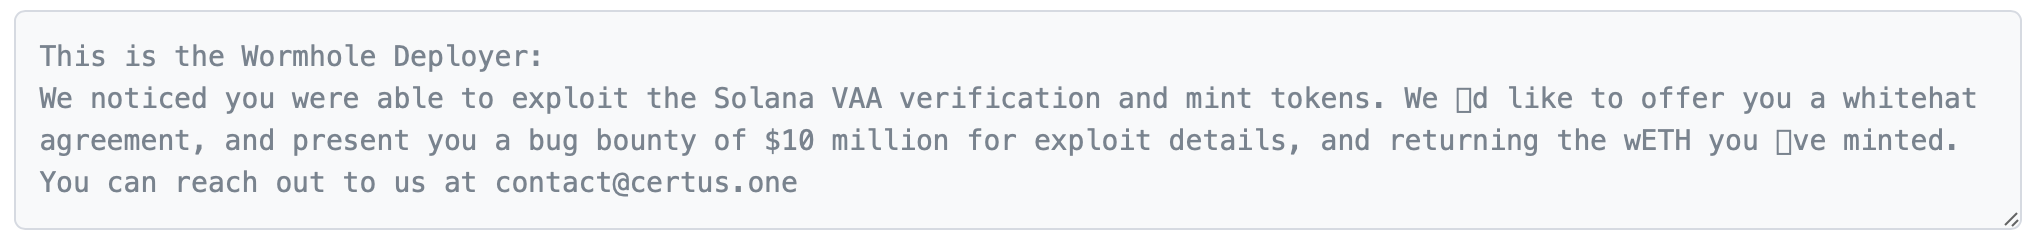
\includegraphics[width=\textwidth]{img/Bounty_offer.png}
\caption{\label{fig:bounty_offer}Chainalysis Reactor graph of the Wormhole hack \cite{hack_schema}}
\end{figure}

\item Jump Trading withdraws 120,000~ETH from an exchange and sends it to Wormhole to cover the stolen funds

The hack led to a state where \$320~million worth of WETH on Solana was unbacked. This imbalance could have resulted in a critical situation as several Solana-based platforms, which accept WETH as collateral, could become insolvent, and users would quickly sell their WETH, both factors accelerating the crash of the value of WETH. The series of events could have resulted in a serious issue for the Solana blockchain and the ecosystem on top of it. 

Luckily, Jump Trading, Wormhole’s parent company and a major player in the Solana ecosystem, withdrew and supplied Ether to replace what was stolen. In the end, there was a 13.5\% dip in Solana’s price shortly after the hack, which may be attribute to concerns around Solana's safety and stability, however, the future of the blockchain and platforms built on top of it remained more or less intact.
\end{enumerate}

\section{Vulnerability Details}

In this section, we will dive deeper into the vulnerability and how exactly the attacker managed to exploit it. 

This part has been written based on information in a series of Tweets by \href{https://twitter.com/samczsun}{samczsun} \cite{samczsun_tweet}.

\begin{enumerate}
\item The attacker created a Solana account \href{https://solscan.io/account/2tHS1cXX2h1KBEaadprqELJ6sV9wLoaSdX68FqsrrZRd}{2tHS1...rrZRd}, which contained a single serialized instruction corresponding to a call to the Secp256k1 contract. 

\item The attacker generated a \texttt{SignatureSet} by calling \texttt{verify\_signatures} and passing in the account created in the previous step as the \texttt{Instruction sysvar}. 

Here lies the core vulnerability that was exploited. The \texttt{verify\_signatures} function is expected to take a set of signatures provided by the guardians and pack it into a \texttt{SignatureSet}. However, it doesn't actually do any verification itself and delegates it to the Secp256k1 program instead, which is the root of the issue. The \texttt{solana\_program::sysvar::instructions} mod should be used with the \texttt{Instruction sysvar}. However, the version of \texttt{solana\_program} that Wormhole used didn't verify the address passed as a parameter. This meant that anyone could create their own account that would hold the same data as the \texttt{Instruction sysvar} and substitute that account for the \texttt{Instruction sysvar} in the \texttt{verify\_signatures} execution. This would essentially bypass signature validation entirely. This way the hacker managed to fully bypass signature validation. The corresponding transaction has the ID \href{https://solscan.io/tx/25Zu1L2Q9uk998d5GMnX43t9u9eVBKvbVtgHndkc2GmUFed8Pu73LGW6hiDsmGXHykKUTLkvUdh4yXPdL3Jo4wVS}{25Zu1...o4wVS}.

\item Next, the hacker executed transaction with ID \href{https://solscan.io/tx/2SohoVoPDSdzgsGCgKQPByKQkLAXHrYmvtE7EEqwKi3qUBTGDDJ7DcfYS7YJC2f8xwKVVa6SFUpH5MZ5xcyn1BCK}{2Soho...n1BCK}, in which the \texttt{post\_vaa} function is called on the main Wormhole bridge. To bypass the signature checks done by this function, the \texttt{SignatureSet} from the previous step was used. This way the hacker was able to generate an acceptable VAA (validator action approval).

\item In the last step of the hack, the attacker executed the \texttt{complete\_wrapped} function with the previously obtained VAA. As a result, the attacker successfully triggered an unauthorized mint and their Solana wallet address received freshly minted 120,000\,ETH in transaction \href{https://solscan.io/tx/2zCz2GgSoSS68eNJENWrYB48dMM1zmH8SZkgYneVDv2G4gRsVfwu5rNXtK5BKFxn7fSqX9BvrBc1rdPAeBEcD6Es}{2zCz2...cD6Es}.

\item After the hack has been completed, the attacker managed to bridge out 10,000\,ETH to their Ethereum wallet address, which can be seen in the transaction with ID \href{https://solscan.io/tx/5UaqPus91wvAzKNve6L8YAHsESomZQ7GWi37gPFyzTHcXNMZA641bb8m8txo7bS7A5cAnzKDKYyiKcQC8GgDcAuf}{5UaqP...DcAuf} on the Solana blockchain and transaction with ID \href{https://etherscan.io/tx/0x4d5201dd4a377f20e61fb8f42e6f929ec16bcec918f0584e39241d15b254a80f}{0x4d520...4a80f} on the Ethereum blockchain.
\end{enumerate}

\section{Conclusion}
We have described and examined the hack of the Wormhole protocol and why it could have had serious consequences. The main lessons we can learn from this attack in order to prevent others in the future are to deploy any significant changes directly after pushing the code to the GitHub repository and to always verify all addresses passed as input.

As of today, the hacker hasn't been identified. Their Ethereum wallet address (0x629e7Da20197\-a5429d30da36E77d06CdF796b71A) still holds 93,750~ETH and their Solana wallet address (CxegPrfn\-2ge5dNiQberUrQJkHCcimeR4VXkeawcFBBka) holds slightly over 432,000 SOL.

\bibliographystyle{ieeetr}
\bibliography{references}

\end{document}
